\documentclass[a4paper,12pt]{article}

\usepackage[]{geometry} 
\usepackage{graphicx}
\usepackage{graphics}
\usepackage{amsmath}
\usepackage{url}
\usepackage{float}
\usepackage{hyperref}
\usepackage{listings}
\usepackage{minted}
\usepackage{pdflscape}
\usepackage{rotating}
\usepackage{mdframed}
\usepackage{wrapfig}
\usepackage{bm}
\usepackage{subcaption}
%\usepackage{fontspec}

\hypersetup{ colorlinks=true, linkcolor=blue, filecolor=magenta, urlcolor=cyan }
\renewcommand\listoflistingscaption{List of source codes}
%\setmonofont{Consolas}

\begin{document}
	
\begin{titlepage}
	\title{
		COMP6223 Computer Vision \\
		\large Subverting Face Detection
	}
	\date{\today}
	\author{
		Ganiyu Ajibola Ibraheem \\
		\large gai1u17@soton.ac.uk \\
			29447267
	}
\end{titlepage}

\maketitle
\newpage
\pagenumbering{roman}
\tableofcontents
\listoffigures
\newpage
\pagenumbering{arabic}


\section{Introduction}
This report highlight the different ways the Viola-Jones Haar Cascade Face detection algorithm can be subverted. This is achieved through applying specially orchestrated make-up at designated parts of the face and also wearing clothing which occludes certain aspects of the face whilst still remaining recognisable by a human.

\section{Subverting by applying make-up on the face}
Taking into account the way the Viola-Jones Haar Cascade Face Detection algorithm (referred to as Face Detection algorithm henceforth) works, one can carefully curate features on the face to trick the algorithm into not detecting a face. \\
	\begin{wrapfigure}{r}{0.5\textwidth} 
		\centering
		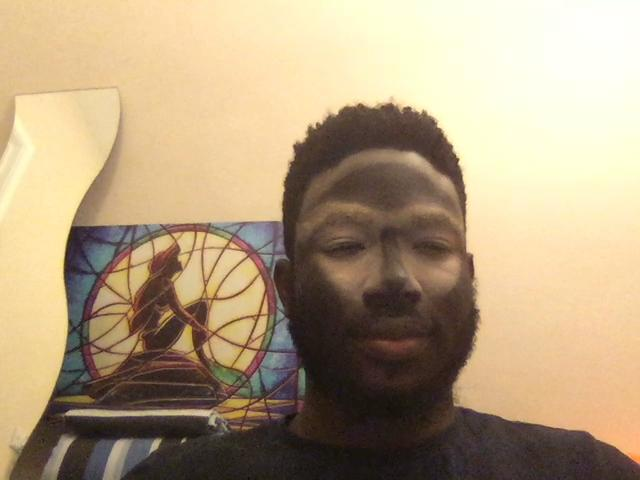
\includegraphics[width=0.6\textwidth]{images/make_up}
		\caption{Applying make-up to subvert the algorithm}
		\label{fig:make_up}
	\end{wrapfigure}
One of the ways this is achieved is with the knowledge that the face detection algorithm uses a window where the average intensity of the rectangular window divided into 3 parts with the middle part being the nose and the other windows being the eyes; it expects a darker region on the sections over the eyes than the section over the nose. \\
	
Taking this into account, white face make-up is applied over the eyes and dark face make-up is applied over the nose bridge. With these special effects applied, when the rectangular window slides over the face, this should create some form of noise over the image resulting in higher intensity values over the eyes and a lower value over the middle section; the algorithm should then misclassify this region. As shown in image \ref{fig:make_up}, there is no bounding box over the face as the algorithm has misclassified this as not a face.

%TODO: Talk about how illumination also affects this value


\section{Subverting by partially occluding the face}
The Face detection algorithm takes into account the location of the eyes, nose and mouth. 
	\begin{figure}[h!]
		\centering
		\begin{subfigure}{0.4\textwidth}
			\centering
			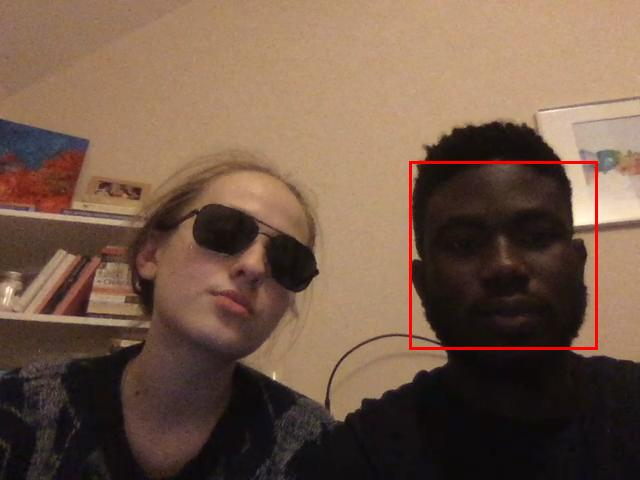
\includegraphics[width=0.9\textwidth]{images/spoof_julia_aj}
			\caption{Partially occluding the face}
			\label{fig:julia}
		\end{subfigure}
		\begin{subfigure}{0.4\textwidth}
			\centering
			
\includegraphics[width=0.9\linewidth]{images/hand_nose}
			\caption{}
			\label{fig:aj_hand}
		\end{subfigure}
		\caption{Viewing images at different scales}
		\label{fig:scales}
	\end{figure}
By partially occluding the face as shown in image \ref{fig:julia} and image \ref{fig:aj_hand}, the algorithm is unable to locate the eyes in the image. This is due to the occlusion of the required features necessary to identify a face such as the dark glasses in image \ref{fig:julia} and the finger over the nose in image \ref{fig:aj_hand}; As these occlusions also affect the intensity values in the targeted parts of the face.


%%\section{Spoofing Approaches}
%%	\begin{itemize}
%%		\item The eye region is darker than the upper-cheeks. To subvert this try white paint around both eyes; check if it detects a face if eyes are opened and closed. Another approach is to make the upper-checks the same complexion as the eye region although this might be harder.
%%		\item The nose bridge region is brighter than the eyes. Can we try making the nose bridge really dark e.g black paint on the nose bridge.
%%		\item Occlusion: The algorithm takes into account the location of the eyes, nose and mouth. Is it possible to use make-up to blend the skin color around these regions to see if it still detects 
%%	\end{itemize}

\section{Conclusion}
Whilst the Viola-Jones algorithm is not the current state of the art, it was one of the first algorithms to run in real time. Numerous algorithms have been further proposed as improvements over the Viola-Jones algorithm such as Feature Point detection, Bag-of-Words models, Histogram-of-oriented gradients (HOG), Deformable Parts Models, Exemplar models and Deep Convolutional Networks with DeepFace by Facebook \cite{latexcompanion} being one of the best performing algorithms.

\begin{thebibliography}{9}
	\bibitem{latexcompanion} 
	Yaniv Taigman, Ming Yang , Marc'Aurelio Ranzato and Lior Wolf.
	\textit{DeepFace: Closing the Gap to Human-Level Performance in Face Verification}. 
	Conference on Computer Vision and Pattern Recognition (CVPR), 2014.
	
\end{thebibliography}


\end{document}